\documentclass{report}

\usepackage{listings}
\usepackage{color}
\usepackage{graphicx}
\usepackage{float}
\usepackage{amsmath}
\usepackage{subfig}
\usepackage{cite}
\usepackage{url}
\usepackage{amsmath}

\begin{document}

\title{3d Graphics - Sea seen from the beach}

\author{Jander Nascimento, 
\and Oleg Iegorov}

\maketitle

\section{Question 1}

\emph{Explain why rendering such a scene is very likely to produce aliasing effects. Will the
deformation of the sea surface due to waves increase or tend to hide these visual problems?}

The horizon that should be displayed in this scenario may produce aliasing due to the procedural modeling (high definition) displayed in a regular sampling \ref{iaow}, looking for it at long distances produces a single color pixel, instead of interpolation of colors. The waves representations may increase the aliasing effect.

\section{Question 2}

\emph{A first idea for modeling the sea surface is to represent it by an initially flat mesh, whose
vertices will be displaced on the vertical axis using z=Height(x,y,t). Two possible flat
quadrangular meshes are considered: a regular 2D grid and a grid computed by projecting the
pixels of the screen onto the horizontal plane of the sea, along the viewing direction (so the
mesh changes each time the camera moves). Which of these representations would you use
and why?}

\section{Question 3}

\emph{Another idea is to directly render the sea surface from the procedural equation of its
geometry Sea(x,y,t) = (x, y, Height(x,y,t)). Which algorithm would you use? Explain the
computations involved on a figure. Can you adapt this algorithm to model specular
reflections while getting real-time performances?}

\section{Question 4}

\emph{The sea model is to be enhanced with some white foam: to simplify the problem, we
suppose that foam is projected forwards from the crest of the waves at a given distance from
the sea shore, falls onto the water surface and then moves with it for a while before
disappearing. How would you animate and render the foam? Give the animation model would
you use, and describe the geometric primitive or the texture it should control, and discuss its
rendering.}

This can me achieved in two steps, first choose the primitive that generate the foam, and the second is to use a tecnique for the foam dynamics (flow). 

Easiest way to render the foam is to use spheres, changing the collision algorithm so they can be displayed as a set of spheres, create foam texture and apply it to the mesh and place it over a certain height, 
But as this looks unrealistic since if a transparency is added to the foam, the intersection between singular bubbles are not natural. 

A more sofisticated method to render the foam is to use Boundary Integral Method to simulate the foam dynamics\cite{bim}. In the figure \ref{fig:dim-foam} we can see an example of a foam generated by this method.

\begin{figure}[H]
\centering
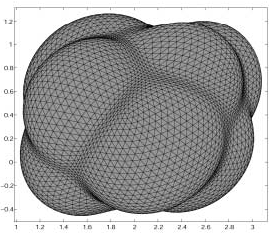
\includegraphics[width=0.4\textwidth]{image/dim01.png}
\caption{Foam rendered by Boundary Integral Method}
\label{fig:dim-foam}
\end{figure}

The transparency is an important aspect of the foam. The transparency can be calculated\cite{nvidia} according to the Equation \ref{equa:transparency}, and apply the acquired value to the geometric primitive used for the foam representation.

\begin{equation}
alpha=saturate(\frac{H-H_0}{H_{max} - H_0})
\label{equa:transparency}
\end{equation}

We can combine the texture with the BIM way of modeling the foam. Apply the texture for further visualization. Since the eye sees a mixed between the colors in long distances, it is possible to apply the texture for saving processing and reduce the aliasing effect.
For a detailed visualization we render the geometric primitive modeled with BIM for the foam.

The foam flow can be computed using two tecniques from dinamical fields (fluid dynamics): surface elevation and potential velocity.

The dynamic aspect of the foam can be modeled using phisically based particle. The particle should respect the gravity, and wind forces until the shore. Based on the elevation of the waves crest defines the speed of the foam. 
The environment conditions for the foam is that the waves must be sufficiently high enough to break and produce the foam(slope greater than 1/6 \cite{sow} of the height of the wave).
When the foam reaches the beach, it should disapear. Removing the particles from outter to the inner layer, simulating the bubble bursted by the wind, since the inner ones are protected the outter bubbles, they tend to burst more easily.

[missing refraction, specular reflaction ]


\begin{thebibliography}{9}

\bibitem{sow}
  Simulating Ocean Water,
  TESSENDORF, Jerry.
  2001

\bibitem{iaow}
  Interactive Animation of Ocean Waves,
  HINSINGER, Damien. NEYRET, Fabrice. CANI, Marie-Paule.
  iMAGIS-GRAVIR

\bibitem{nvidia}
  Interactive Animation of Ocean Waves,
  Kryachko,Yuri.
  GPU Gems 2. 
  Second printing, April 2005.
  \url{http://http.developer.nvidia.com/GPUGems2/gpugems2_chapter18.html}

\bibitem{bim}
  Boundary Integral for 3d Simulation of Foam Dynamics,
  Ivan B. Bazhlekov, Frans N. van de Vosse, and Han E.H. Meijer.
  Eindhoven University of Technology.

\end{thebibliography}



\end{document}


